\section{Introduction}\label{introduction}


\begin{frame}{Motivation}

	\begin{itemize}
		\item
		Renewable energy scenarios are important in many fields in Power
		Systems:
		
		\begin{enumerate}
			\def\labelenumi{\roman{enumi})}
			
			\item
			Energy trading;
			\item
			unit commitment;
			\item
			grid expansion planning;
			\item
			investment decisions
		\end{enumerate}
		\item
		In stochastic optimization problems, a set of scenarios is a needed
		input.
		\item
		Robust optimization requires bounds for probable values.
	\end{itemize}

	\textbf{Change in paradigm: from predicting the conditional mean to
		predicting the conditional distribution}

\end{frame}



\begin{frame}{Probability Forecasting Approaches}

	\begin{itemize}

	\item
	\emph{Parametric Models}

	\begin{itemize}
		
		\item
		Assume a distributional shape
		\item
		Low computational costs
		\item
		Faster convergence
		\item
		\emph{Examples: Arima-GARCH, GAS}
	\end{itemize}
	\item
	\emph{Nonparametric Models}

	\begin{itemize}
		
		\item
		Don't require a distribution to be specified
		\item
		High computational cost
		\item
		Needs more data to produce a good approximation

		\item Examples: Quantile Regression \cite{koenker1978regression}, Kernel Density Estimation \cite{gallego2016line} and Artificial Inteligende \cite{Wan2017}.
	\end{itemize}
	\end{itemize}

\end{frame}


\begin{frame}{Wind Power Time Series - Icaraizinho monthly data}

	\begin{figure}
	\centering
	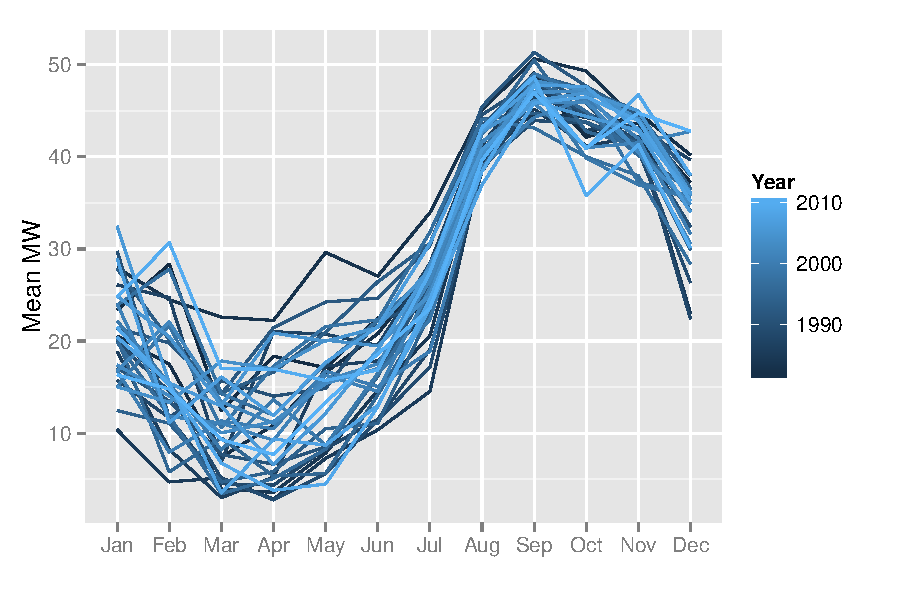
\includegraphics[width=0.9\linewidth]{Images/icaraizinho-mensal}
	\end{figure}

\end{frame}


\begin{frame}{Wind Power Time Series - Kaggle forecasting competition hourly data}

	\begin{figure}
	\centering
	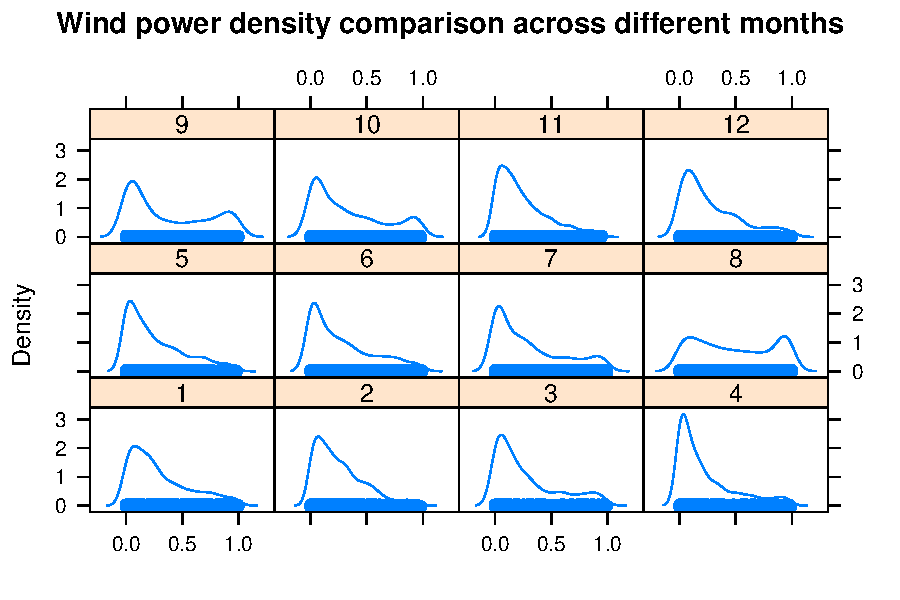
\includegraphics[width=0.9\linewidth]{Images/density}
	\end{figure}

\end{frame}

\begin{frame}{The nongaussianity of Wind Power}

	\begin{itemize}
	
	\item
	Renewables, such as wind and solar power have reportedly nongaussian behaviour.
	\item
	Convenience of using a nonparametric approach, which doesn't rely on assuming a distribution.
	\item
	Quantile regression is the chosen technique available to model this time series dynamics, by estimating a thin grid of $\alpha$-quantiles at once and forming a data-driven conditional distribution
	\end{itemize}
	
\end{frame}


\begin{frame}{Scenario Simulation}

	\begin{itemize}
		\item In order to simulate scenarios, not only the conditional mean is needed, but the whole conditional distribution, whose estimation procedure is the most important contribution in this work.
		
		\item The procedure is drawing, in each period $\tau$, a value for $\tau+1$ from the estimated conditional distribution function (CDF). Hence, having a good estimate of the CDF is essential to meet the goal in this work. 

		\todo{Put a simulation graph}

	\end{itemize}
\end{frame}



\begin{frame}{Building an estimator of the CDF}
	\begin{itemize}
		\item Construct the CDF nonparametrically by using a sequence of quantile values $q_\alpha$ by estimating many quantiles on a thin grid of probabilities over the interval $[0,1]$. 
		
		\item Transforming this set of points $q_{\alpha_1}, q_{\alpha_2}, \dots, q_{\alpha_{|J|}}$ into a continuous function by using a interpolating method. 

		\todo{Picture with points}
	\end{itemize}
	% These quantile values may be estimated by a technique such as Quantile Regression (QR). 
	% The seminal work \cite{koenker1978regression} defines QR as it is employed in many works \cite{chao_quantile_2012,li_quantile_2007,bosch_convergent_nodate,gallego2016line,moller_time-adaptive_2008,nielsen2006,bremnes_probabilistic_2004,wan_direct_2017}. The conditional quantile is the solution of an optimization problem where the sum of the check function (defined formally in the next session) is minimized. Instead of using the classical regression to estimate the conditional mean, QR determines any quantile from the conditional distribution. Applications are enormous, ranging from risk measuring at financial funds (the Value-at-Risk) to a central measure robust to outliers.
\end{frame}


\begin{frame}{Quantile Regression}
	\begin{itemize}
		\item Defined by \cite{koenker1978regression} as the solution of the following minimization problem 
			\begin{equation}
				\underset{q\in\mathcal{Q}}{\text{min}}\, L_\alpha(q) = \sum_{t\in T}\rho_{\alpha}(y_{t}-q(x_t)),\label{eq:optim-lqr1} 
			\end{equation}
			where
			\begin{equation}\label{eq:check-function}
				\rho_{\alpha}(x)=\begin{cases}
				\alpha x & \text{if }x\geq0\\
				(1-\alpha)x & \text{if }x<0
				\end{cases}.
			\end{equation}
	\end{itemize}
\end{frame}


\begin{frame}{QR to model Wind Power Time Series}
	\begin{itemize}
		\item \cite{moller_time-adaptive_2008}: updating quantile regression model.
		\item \cite{nielsen2006}: builds a quantile model using already existent independent forecasts.
		\item \cite{gallego-castillo_-line_2016}: uses nonparametric QR with a Reproducing Kernel Hilbert Space.
		\item \cite{wan2016}: Neural network with one hidden layer (extreme learning machine) to forecast quantiles.
	\end{itemize}
\end{frame}

\begin{frame}{Blau}
\begin{figure}
\begin{center}
	\includegraphics[width=0.7\linewidth,height=0.7\textheight,keepaspectratio]{pg_0004}
\end{center}
\caption{ADA}
\end{figure}
\end{frame}

\begin{frame}{Blau2}
	\begin{figure}
	\begin{center}
		\includegraphics[width=0.7\textwidth]{pg_0004}
	\end{center}
	\caption{eki}
	\end{figure}
\end{frame}
	


\begin{frame}{Proposed methodology to estimate the Conditional Density Function}
\begin{figure}
\begin{center}
	\includegraphics[width=0.75\textwidth]{Images/Diagrama-trabalho}
\end{center}
\end{figure}
\end{frame}






\begin{frame}{Objectives}
	\begin{itemize}
		\item A nonparametric methodology to model, from a set of quantile estimations, the conditional distribution of RG time series to produce future scenarios.
		
		\item The proposition of two different procedures to jointly estimate quantiles: (i) A linear model that selects the global optimal solution with parsimony both on the selection of covariates as on the quantiles. This methodology is based on the Adaptive LASSO for QR (Linear Programming). (ii) A nonparametric quantile regression model, which has a free functional form, tuned by a penalty on how rough this function may be. 
		
		\item Regularization techniques applied to an ensemble of quantile functions to estimate the conditional distribution, solving the issue of non-crossing quantiles. On regularizing quantiles, we propose a smoothness on the coefficient value across the sequence of quantiles.
		%\item A nonlinear QR
		
	\end{itemize}
	
\end{frame}
